%============================================================
%  Capitolo 8 – Reti Ricorrenti
%============================================================
\chapter{Reti Ricorrenti}
\label{ch:recurrent-networks}

I dati del mondo reale sono spesso intrinsecamente \emph{sequenziali}: la
posizione futura di un oggetto in moto, le parole di un testo, le note di una
melodia o i fotogrammi di un video dipendono da ciò che è accaduto
\emph{prima}. Le reti neurali standard (feed-forward) ignorano questa struttura
temporale: ricevono un input di dimensione fissa e producono un output
indipendente da ogni elaborazione precedente. Le \textbf{reti neurali
ricorrenti} (RNN) colmano questa lacuna introducendo un meccanismo di
\emph{memoria implicita} che trasmette informazioni da un passo temporale al
successivo \citep{bishop2024}.

%------------------------------------------------------------
\section{Motivazione: Modellare Sequenze}
\label{sec:rnn-motivation}

\subsection{Il Problema della Modellazione Sequenziale}
\label{subsec:seq-problem}

Consideriamo il compito di predire la prossima parola in una frase. Un primo
approccio naïve consiste nell'usare una finestra fissa di $k$ parole precedenti
come input a una rete feed-forward (\emph{fixed-window approach}). Questo schema
soffre però di tre limitazioni fondamentali:

\begin{description}
  \item[Dipendenze a lungo termine] Una finestra fissa non può catturare
        contesti lontani nel tempo. Frase come \emph{``France is where I grew
        up, but I now live in Boston. I speak fluent \underline{\hspace{1cm}}''}
        richiedono informazioni che si trovano decine di parole prima.
  \item[Mancato rispetto dell'ordine] La rappresentazione a \emph{bag of words}
        codifica solo la presenza/assenza di parole: non distingue \emph{``The
        food was good, not bad at all''} da \emph{``The food was bad, not good
        at all''}.
  \item[Assenza di condivisione dei parametri] Con una finestra grande ogni
        posizione ha i propri pesi separati; ciò impedisce di trasferire le
        conoscenze apprese in una posizione alle altre.
\end{description}

Le RNN risolvono questi problemi mantenendo uno \textbf{stato nascosto}
$\mathbf{h}_t$ che riassume tutta la storia della sequenza fino al passo $t$.

\subsection{Rappresentazione Numerica del Linguaggio}
\label{subsec:word-embedding}

Le reti neurali richiedono input numerici; le parole devono essere quindi
trasformate in vettori. Il processo si articola in tre fasi: costruire un
\textbf{vocabolario} (corpus di tutte le parole), assegnare un indice a ogni
parola (\textbf{indicizzazione}), e infine convertire l'indice in un vettore di
dimensione fissa tramite \textbf{embedding}.

\begin{figure}[H]
  \centering
  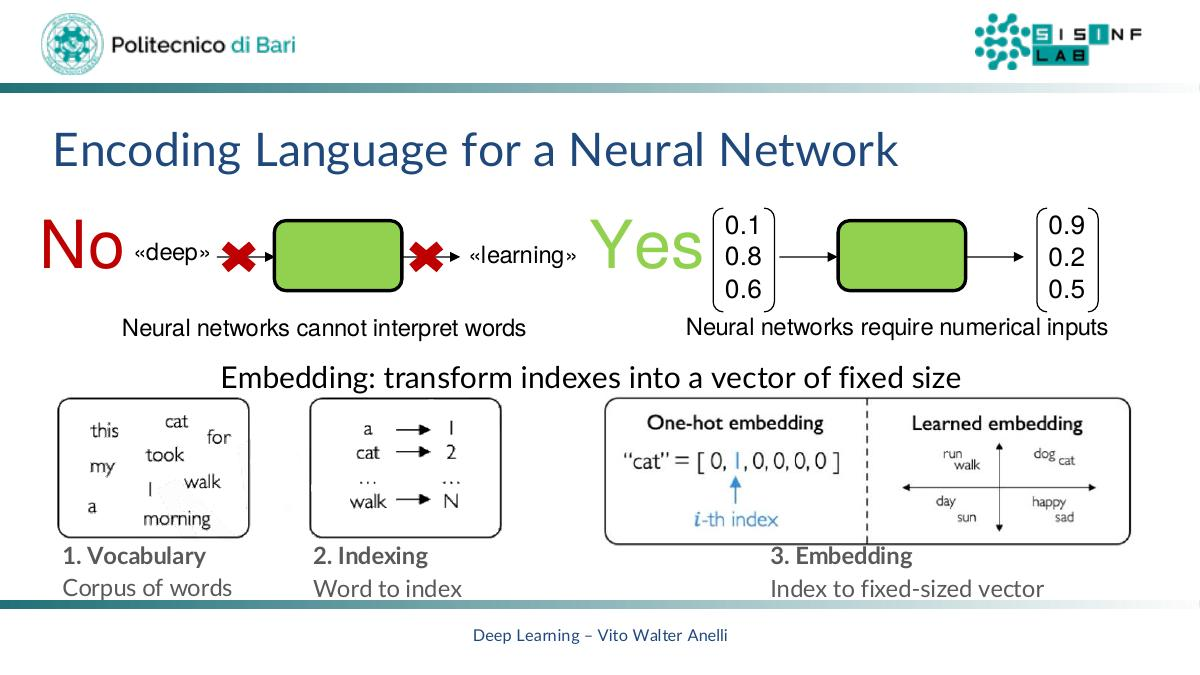
\includegraphics[width=0.82\linewidth]{figures/cf08_word_embedding.jpg}
  \caption{Codifica del linguaggio per una rete neurale. Sinistra: le parole non
           possono essere date direttamente in input. Centro: one-hot encoding
           (sparso, non apprende similarità semantiche). Destra: learned
           embedding (denso, cattura relazioni tra parole nello spazio
           vettoriale).}
  \label{fig:word_embedding}
\end{figure}

L'\textbf{one-hot encoding} rappresenta la parola $i$ come un vettore binario
di lunghezza $|V|$ con un solo 1 nella posizione $i$; è semplice ma non codifica
alcuna nozione di similarità semantica. Il \textbf{learned embedding} (es.
Word2Vec, GloVe) apprende durante l'addestramento una matrice
$E \in \mathbb{R}^{|V| \times d}$ che proietta ogni indice in un vettore denso
di dimensione $d$, catturando relazioni semantiche come
$\text{king} - \text{man} + \text{woman} \approx \text{queen}$.

%------------------------------------------------------------
\section{Reti Neurali Ricorrenti (RNN)}
\label{sec:rnn}

\subsection{Neuroni con Ricorrenza}
\label{subsec:neurons-recurrence}

Una rete feed-forward calcola $\hat{\mathbf{y}}_t = f(\mathbf{x}_t)$
indipendentemente per ogni passo temporale. Una \textbf{RNN} invece aggiunge
una connessione ricorrente dallo stato nascosto al passo precedente:

\begin{equation}
  \hat{\mathbf{y}}_t = f(\mathbf{x}_t,\, \mathbf{h}_{t-1}).
  \label{eq:rnn-output}
\end{equation}

L'equazione di \textbf{aggiornamento dello stato nascosto} e di
\textbf{produzione dell'output} di una RNN vanilla sono:

\begin{align}
  \mathbf{h}_t &= \tanh\!\left(W_{hh}^{T}\,\mathbf{h}_{t-1}
                   + W_{xh}^{T}\,\mathbf{x}_t\right),
  \label{eq:rnn-hidden} \\
  \hat{\mathbf{y}}_t &= W_{hy}^{T}\,\mathbf{h}_t,
  \label{eq:rnn-output2}
\end{align}

dove $W_{hh} \in \mathbb{R}^{d_h \times d_h}$, $W_{xh} \in \mathbb{R}^{d_x
\times d_h}$ e $W_{hy} \in \mathbb{R}^{d_h \times d_y}$ sono le matrici dei
pesi, \emph{condivise tra tutti i passi temporali}. Questa condivisione è la
chiave dell'efficienza parametrica delle RNN.

\begin{figure}[H]
  \centering
  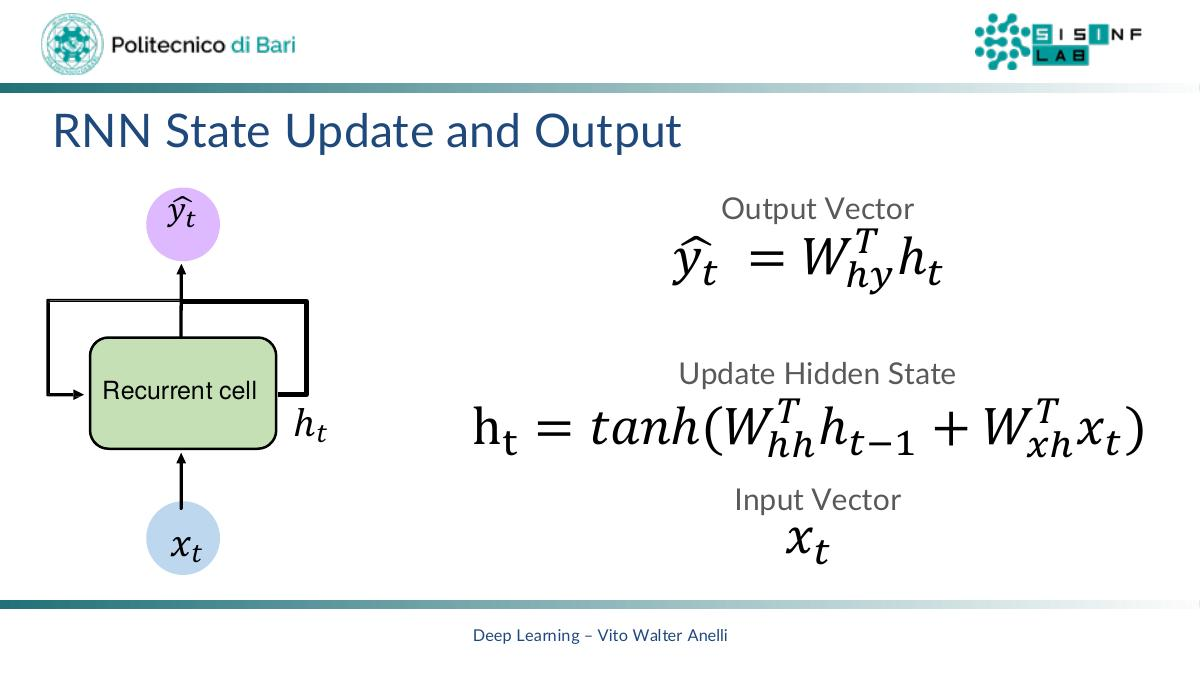
\includegraphics[width=0.82\linewidth]{figures/cf08_rnn_state_update.jpg}
  \caption{Cella ricorrente: sinistra, la rappresentazione compatta con il loop
           di ricorrenza; destra, le equazioni di aggiornamento dello stato
           nascosto $\mathbf{h}_t$ e di calcolo dell'output $\hat{\mathbf{y}}_t$.}
  \label{fig:rnn_state_update}
\end{figure}

\paragraph{Implementazione in PyTorch.}
\begin{lstlisting}[language=Python, caption={RNN minima in PyTorch.}, label={lst:rnn-pytorch}]
import torch.nn as nn

rnn = nn.RNN(input_size=d_x, hidden_size=d_h,
             num_layers=1, batch_first=True)
# output: (batch, seq_len, d_h), h_n: (1, batch, d_h)
output, h_n = rnn(x, h_0)
\end{lstlisting}

\subsection{Grafo Computazionale nel Tempo}
\label{subsec:unrolled-graph}

Una RNN può essere visualizzata come una rete feed-forward molto profonda
ottenuta \emph{srotolando} (\emph{unrolling}) la ricorrenza nel tempo. Ad ogni
passo temporale si inserisce un livello che condivide i pesi con tutti gli
altri. La loss totale è la somma delle loss ai singoli istanti:

\begin{equation}
  \mathcal{L} = \sum_{t=0}^{T} \mathcal{L}_t\!\left(\hat{\mathbf{y}}_t,
  \mathbf{y}_t\right).
  \label{eq:rnn-total-loss}
\end{equation}

\begin{figure}[H]
  \centering
  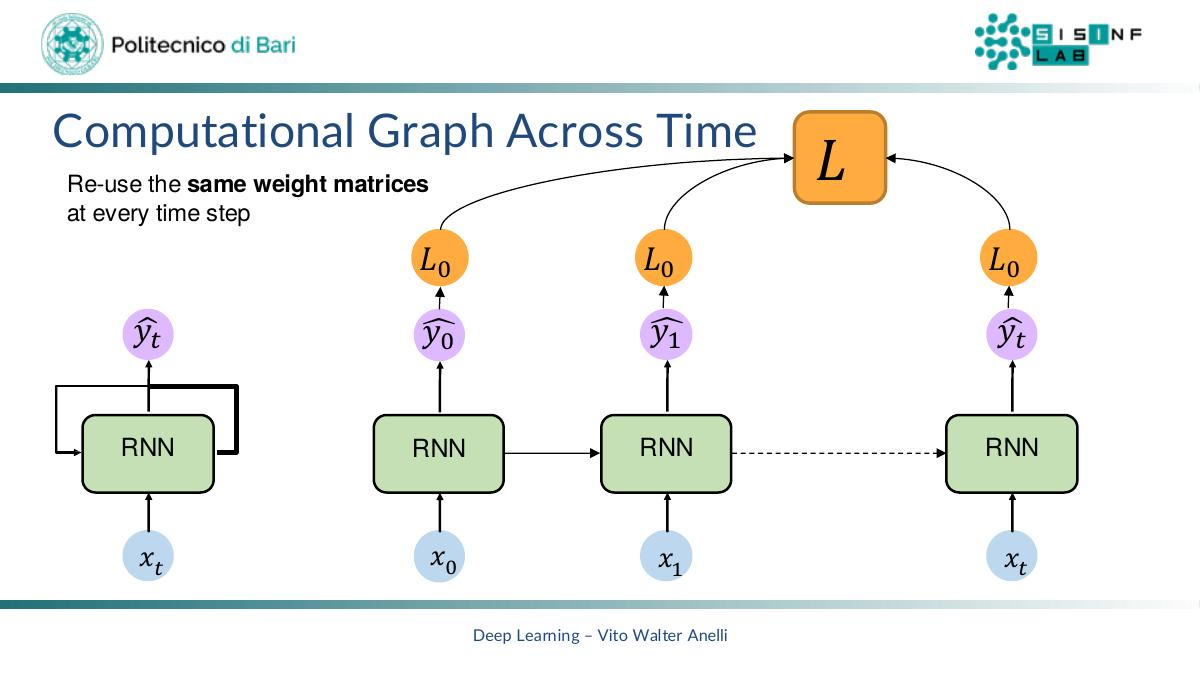
\includegraphics[width=0.82\linewidth]{figures/cf08_rnn_unrolled.jpg}
  \caption{Grafo computazionale di una RNN srotolato nel tempo. Le stesse
           matrici dei pesi $W_{hh}$, $W_{xh}$, $W_{hy}$ vengono riusate a ogni
           passo; la loss $\mathcal{L}$ è la somma delle loss parziali
           $\mathcal{L}_0, \mathcal{L}_1, \ldots$}
  \label{fig:rnn_unrolled}
\end{figure}

\subsection{Architetture Sequenziali}
\label{subsec:rnn-architectures}

A seconda del rapporto tra lunghezza dell'input e dell'output si distinguono:

\begin{description}
  \item[One-to-One] Rete vanilla senza ricorrenza.
  \item[Many-to-One] Una sequenza in ingresso produce un singolo output
        (es.\ classificazione del sentiment).
  \item[One-to-Many] Un singolo input produce una sequenza in uscita
        (es.\ generazione di musica o di testo).
  \item[Many-to-Many] Sequenza in ingresso, sequenza in uscita (es.\
        traduzione automatica, etichettatura POS).
\end{description}

%------------------------------------------------------------
\section{Backpropagation Through Time (BPTT)}
\label{sec:bptt}

\subsection{Algoritmo}
\label{subsec:bptt-algorithm}

Poiché la RNN srotolata è equivalente a una rete feed-forward con pesi
condivisi, la si può addestrare con la normale backpropagation applicata al
grafo computazionale nel tempo: è il cosiddetto algoritmo di
\textbf{Backpropagation Through Time (BPTT)} \citep{bishop2024}.

\begin{itemize}
  \item Il \emph{forward pass} scorre la sequenza da $t=0$ a $t=T$,
        costruendo uno stack delle attività nascoste $\mathbf{h}_0, \ldots,
        \mathbf{h}_T$.
  \item Il \emph{backward pass} disimpila le attività e calcola i gradienti
        dell'errore a ogni passo temporale.
  \item I gradienti rispetto a $W_{hh}$, $W_{xh}$, $W_{hy}$ vengono sommati
        su tutti i passi prima dell'aggiornamento.
\end{itemize}

Formalmente, il gradiente dell'errore rispetto allo stato nascosto al passo $t$
dipende da tutti i passi successivi:

\begin{equation}
  \frac{\partial \mathcal{L}}{\partial \mathbf{h}_t} =
  \frac{\partial \mathcal{L}_t}{\partial \mathbf{h}_t} +
  \frac{\partial \mathcal{L}}{\partial \mathbf{h}_{t+1}}
  \frac{\partial \mathbf{h}_{t+1}}{\partial \mathbf{h}_t}.
\end{equation}

\subsection{Il Problema dei Gradienti che Svaniscono o Esplodono}
\label{subsec:vanishing-exploding}

Il calcolo del gradiente rispetto allo stato nascosto iniziale $\mathbf{h}_0$
richiede il prodotto di $T$ fattori $W_{hh}$ (moltiplicazione matriciale
ripetuta). Questo genera due patologie simmetriche:

\begin{description}
  \item[Gradienti che svaniscono] Se i valori singolari di $W_{hh}$ sono
        $< 1$, il prodotto converge a zero esponenzialmente: le informazioni
        distanti nel tempo non riescono più a influenzare i pesi.
  \item[Gradienti che esplodono] Se i valori singolari sono $> 1$, il prodotto
        diverge: l'addestramento diventa instabile.
\end{description}

\begin{figure}[H]
  \centering
  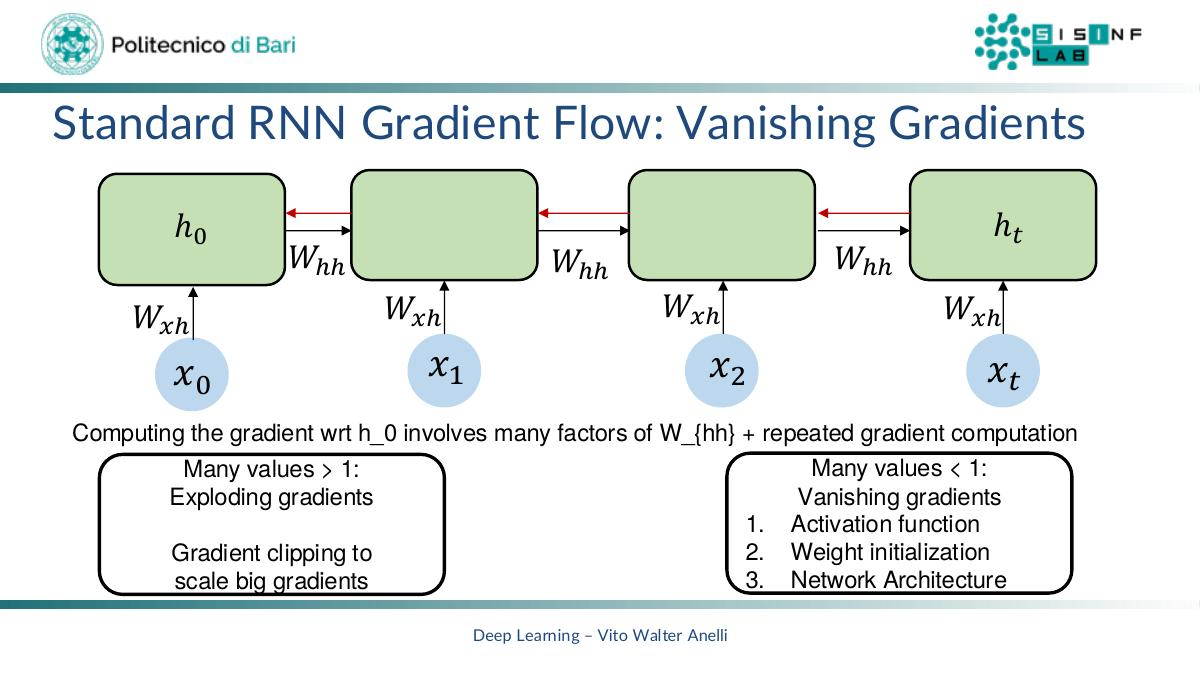
\includegraphics[width=0.82\linewidth]{figures/cf08_vanishing_gradients.jpg}
  \caption{Flusso del gradiente in una RNN standard. Le frecce rosse mostrano
           come il gradiente debba attraversare molte moltiplicazioni per
           $W_{hh}$ per raggiungere $\mathbf{h}_0$. Se $\|W_{hh}\| < 1$:
           vanishing; se $\|W_{hh}\| > 1$: exploding.}
  \label{fig:vanishing_gradients}
\end{figure}

\paragraph{Soluzioni pratiche.}
\begin{itemize}
  \item \textbf{Gradient clipping}: si riscalano i gradienti quando la loro
        norma supera una soglia $\theta$:
        $\nabla \leftarrow \frac{\theta}{\|\nabla\|}\,\nabla$ se
        $\|\nabla\| > \theta$. Mitiga l'esplosione.
  \item \textbf{Inizializzazione della matrice $W_{hh}$} come matrice ortogonale
        (valori singolari = 1): rallenta il collasso.
  \item \textbf{Architetture con gate} (LSTM, GRU): soluzione strutturale
        al problema del vanishing (Sezione \ref{sec:lstm}).
\end{itemize}

\paragraph{Nota sul backward pass lineare.}
A differenza del forward pass — dove funzioni di attivazione come $\tanh$
saturano e \emph{comprimono} i valori — il backward pass è localmente
\emph{lineare}: raddoppiare i gradienti all'uscita raddoppia tutti i gradienti
a ritroso nella rete. Questo amplifica la fragilità numerica del BPTT su
sequenze lunghe.

%------------------------------------------------------------
\section{Long Short-Term Memory (LSTM)}
\label{sec:lstm}

\subsection{Motivazione: La Memoria Analogica}
\label{subsec:lstm-motivation}

\citet{hochreiter1997lstm} propongono di risolvere il problema del vanishing
gradient introducendo una \textbf{cella di memoria} con connessioni lineari
di auto-rinforzo (peso di auto-collegamento uguale a 1) e \textbf{porte}
(\emph{gates}) che controllano selettivamente la scrittura, la lettura e la
cancellazione delle informazioni.

\begin{figure}[H]
  \centering
  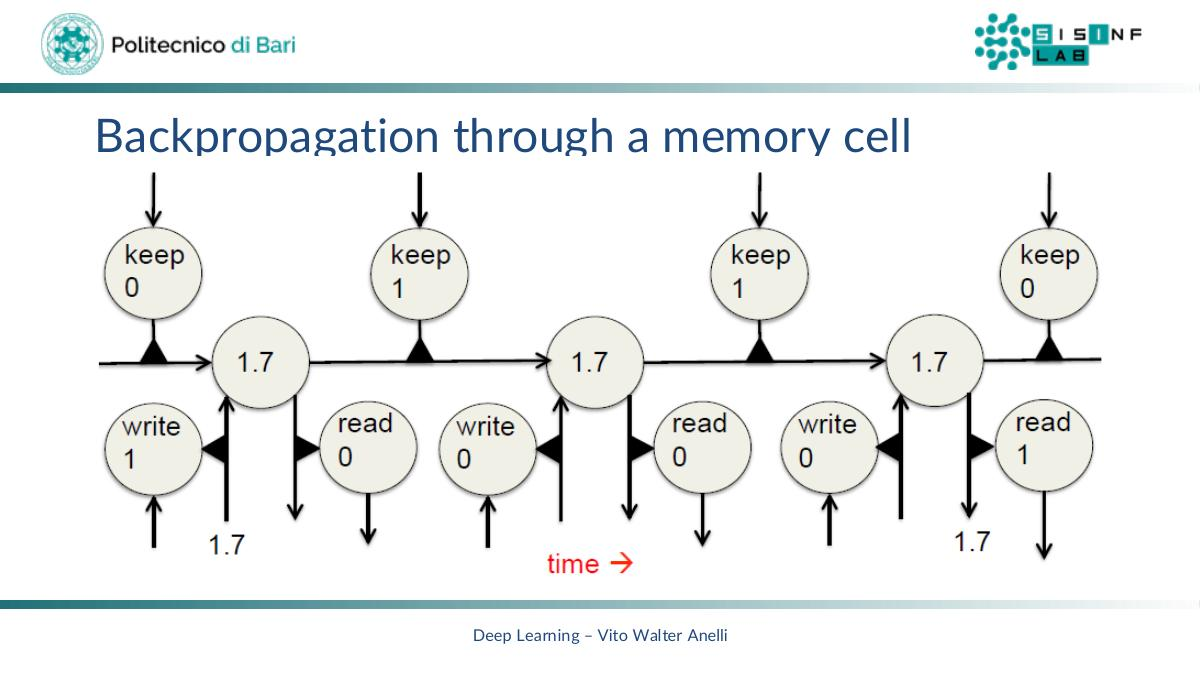
\includegraphics[width=0.82\linewidth]{figures/cf08_memory_cell_bptt.jpg}
  \caption{Cella di memoria analogica: il valore 1.7 viene scritto quando il
           gate \emph{write}~=~1, mantenuto finché \emph{keep}~=~1, e letto
           quando \emph{read}~=~1. La backpropagation attraversa questo
           circuito perché le porte logistiche hanno derivate ben definite.}
  \label{fig:memory_cell}
\end{figure}

\subsection{Architettura della Cella LSTM}
\label{subsec:lstm-architecture}

Una cella LSTM mantiene due vettori di stato distinti:
\begin{itemize}
  \item $\mathbf{c}_t \in \mathbb{R}^{d_h}$: \textbf{cell state}, la memoria
        a lungo termine.
  \item $\mathbf{h}_t \in \mathbb{R}^{d_h}$: \textbf{hidden state}, la memoria
        a breve termine e l'output della cella.
\end{itemize}

\begin{figure}[H]
  \centering
  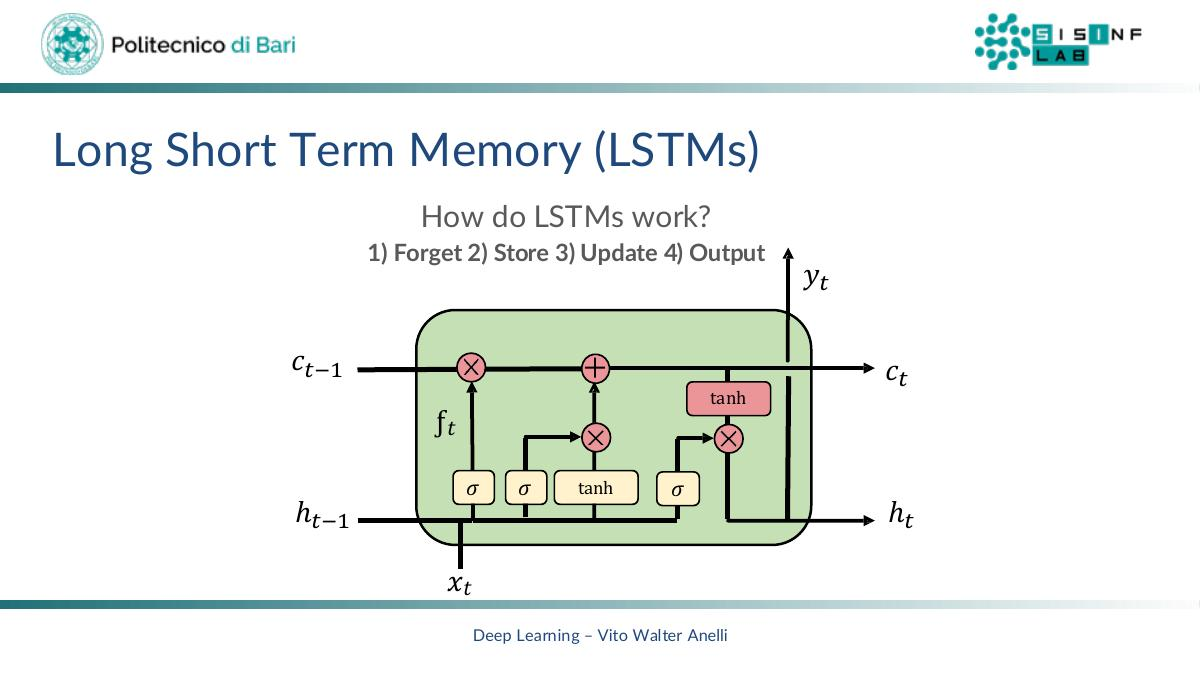
\includegraphics[width=0.75\linewidth]{figures/cf08_lstm_full.jpg}
  \caption{Schema completo della cella LSTM. Il cell state $\mathbf{c}_t$
           scorre orizzontalmente subendo solo operazioni element-wise
           (moltiplicazione e addizione), garantendo un flusso del gradiente
           non interrotto durante la BPTT.}
  \label{fig:lstm_full}
\end{figure}

Il comportamento della cella si articola in quattro fasi.

\subsubsection{Forget Gate (Cancellazione)}
\label{subsubsec:forget-gate}

Il forget gate decide quali informazioni eliminare dallo stato della cella:

\begin{equation}
  \mathbf{f}_t = \sigma\!\left(W_f \begin{bmatrix}\mathbf{h}_{t-1}\\
  \mathbf{x}_t\end{bmatrix} + \mathbf{b}_f\right),
  \label{eq:forget-gate}
\end{equation}

dove $\sigma$ è la sigmoide. Un valore $f_t^{(i)} \approx 0$ cancella
l'$i$-esima componente del cell state; $f_t^{(i)} \approx 1$ la conserva.

\begin{figure}[H]
  \centering
  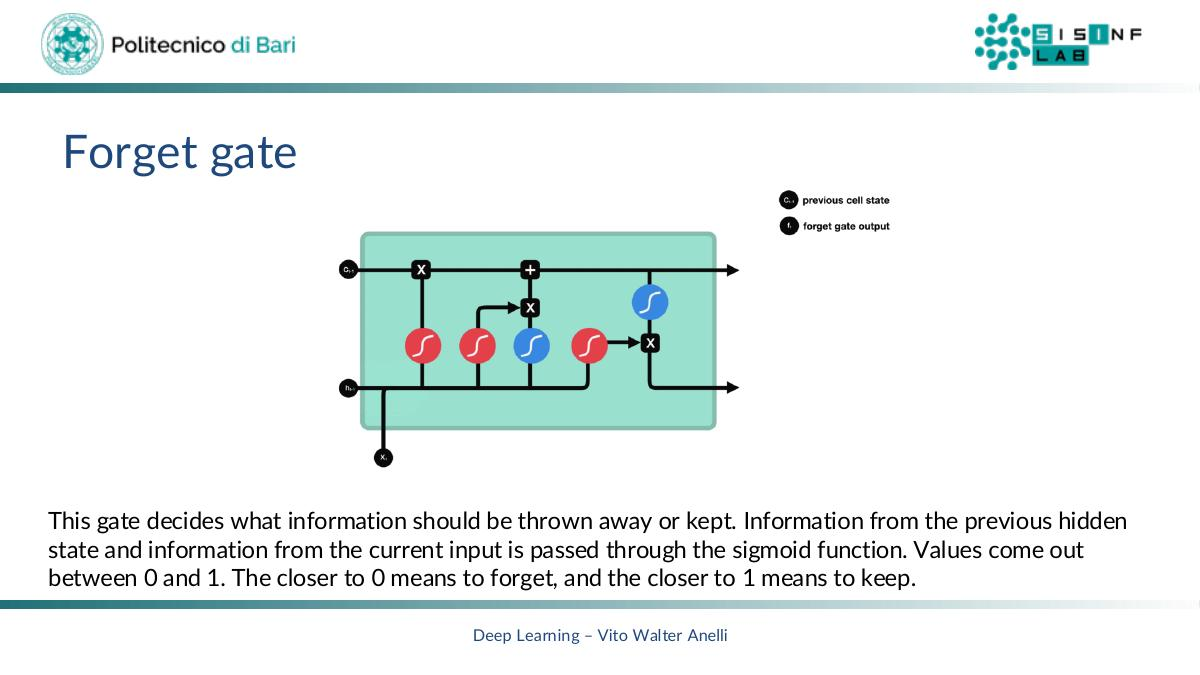
\includegraphics[width=0.70\linewidth]{figures/cf08_lstm_forget_gate.jpg}
  \caption{Forget gate: le attivazioni sigmoidee (in rosso) determinano quali
           informazioni del cell state precedente vengono eliminate (moltiplicazione
           per $\mathbf{f}_t$).}
  \label{fig:lstm_forget}
\end{figure}

\subsubsection{Input Gate (Memorizzazione)}
\label{subsubsec:input-gate}

Due sub-gate cooperano per aggiungere nuova informazione al cell state:

\begin{align}
  \mathbf{i}_t &= \sigma\!\left(W_i \begin{bmatrix}\mathbf{h}_{t-1}\\
                    \mathbf{x}_t\end{bmatrix} + \mathbf{b}_i\right),
  \label{eq:input-gate} \\
  \tilde{\mathbf{c}}_t &= \tanh\!\left(W_c \begin{bmatrix}\mathbf{h}_{t-1}\\
                    \mathbf{x}_t\end{bmatrix} + \mathbf{b}_c\right).
  \label{eq:candidate-cell}
\end{align}

$\mathbf{i}_t$ (gate sigmoid) seleziona quali componenti aggiornare;
$\tilde{\mathbf{c}}_t$ (gate tanh) genera il valore candidato da scrivere.

\subsubsection{Aggiornamento del Cell State}
\label{subsubsec:cell-update}

Il cell state viene aggiornato combinando la cancellazione e la scrittura
selettiva:

\begin{equation}
  \mathbf{c}_t = \mathbf{f}_t \odot \mathbf{c}_{t-1}
                + \mathbf{i}_t \odot \tilde{\mathbf{c}}_t,
  \label{eq:cell-update}
\end{equation}

dove $\odot$ indica il prodotto element-wise (Hadamard).

\subsubsection{Output Gate (Uscita)}
\label{subsubsec:output-gate}

L'output gate filtra il cell state per produrre il nuovo hidden state:

\begin{align}
  \mathbf{o}_t &= \sigma\!\left(W_o \begin{bmatrix}\mathbf{h}_{t-1}\\
                    \mathbf{x}_t\end{bmatrix} + \mathbf{b}_o\right),
  \label{eq:output-gate} \\
  \mathbf{h}_t &= \mathbf{o}_t \odot \tanh(\mathbf{c}_t).
  \label{eq:hidden-output}
\end{align}

\subsection{Flusso del Gradiente nelle LSTM}
\label{subsec:lstm-gradient}

Il punto cruciale delle LSTM è che la backpropagation da $\mathbf{c}_t$ a
$\mathbf{c}_{t-1}$ richiede \emph{solo operazioni element-wise} (moltiplicazione
per $\mathbf{f}_t$ e addizione); non c'è alcuna moltiplicazione matriciale lungo
il percorso del cell state. Di conseguenza:

\begin{itemize}
  \item Il gradiente scorre quasi indisturbato per centinaia di passi temporali
        (\emph{uninterrupted gradient flow}).
  \item Il forget gate impara a modulare il decay del gradiente in modo
        \emph{adattivo}: quando $\mathbf{f}_t \approx \mathbf{1}$ il gradiente
        viene interamente preservato; quando $\mathbf{f}_t \approx \mathbf{0}$
        la dipendenza dal passato viene eliminata.
\end{itemize}

\begin{lstlisting}[language=Python, caption={LSTM in PyTorch.}, label={lst:lstm-pytorch}]
import torch.nn as nn

lstm = nn.LSTM(input_size=d_x, hidden_size=d_h,
               num_layers=n_layers, batch_first=True)
# h_0, c_0: (n_layers, batch, d_h)
output, (h_n, c_n) = lstm(x, (h_0, c_0))
\end{lstlisting}

%------------------------------------------------------------
\section{Gated Recurrent Unit (GRU)}
\label{sec:gru}

\subsection{Architettura}
\label{subsec:gru-architecture}

La \textbf{Gated Recurrent Unit} \citep{cho2014gru} è una semplificazione delle
LSTM che elimina il cell state separato e usa solo due porte, riducendo il numero
di parametri e spesso raggiungendo prestazioni comparabili.

\paragraph{Reset gate.}
Il reset gate $\mathbf{r}_t$ controlla quanta memoria del passato viene
dimenticata nel calcolo del candidato:

\begin{equation}
  \mathbf{r}_t = \sigma\!\left(W_r\,[\mathbf{h}_{t-1};\,\mathbf{x}_t]
                 + \mathbf{b}_r\right).
  \label{eq:gru-reset}
\end{equation}

\paragraph{Update gate.}
Il update gate $\mathbf{z}_t$ determina in che misura il candidato
$\tilde{\mathbf{h}}_t$ sostituisce il vecchio hidden state:

\begin{equation}
  \mathbf{z}_t = \sigma\!\left(W_z\,[\mathbf{h}_{t-1};\,\mathbf{x}_t]
                 + \mathbf{b}_z\right).
  \label{eq:gru-update}
\end{equation}

\begin{figure}[H]
  \centering
  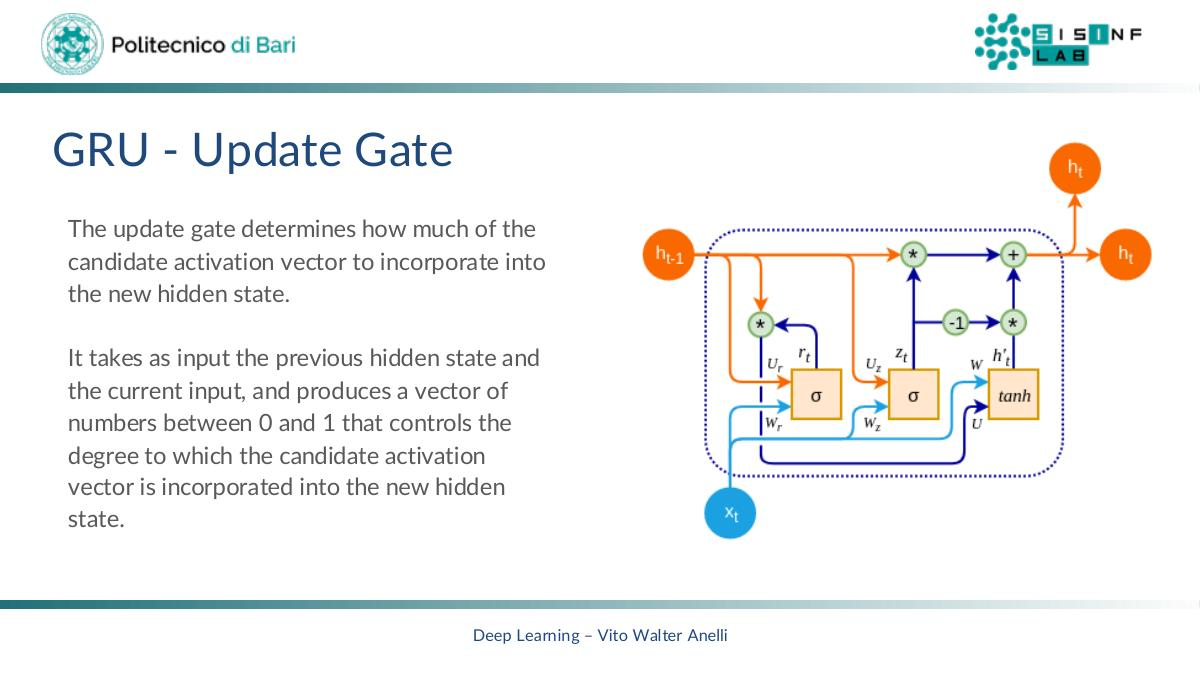
\includegraphics[width=0.72\linewidth]{figures/cf08_gru_update_gate.jpg}
  \caption{GRU: update gate $\mathbf{z}_t$ (a destra nel diagramma). Il
           vettore di output è una media pesata tra il vecchio stato e il
           candidato, con il bilanciamento controllato da $\mathbf{z}_t$.}
  \label{fig:gru_update}
\end{figure}

\paragraph{Candidato e aggiornamento.}

\begin{align}
  \tilde{\mathbf{h}}_t &= \tanh\!\left(W\,[\mathbf{r}_t \odot
                           \mathbf{h}_{t-1};\, \mathbf{x}_t]
                           + \mathbf{b}\right),
  \label{eq:gru-candidate} \\
  \mathbf{h}_t &= (\mathbf{1} - \mathbf{z}_t) \odot \mathbf{h}_{t-1}
                + \mathbf{z}_t \odot \tilde{\mathbf{h}}_t.
  \label{eq:gru-final}
\end{align}

L'equazione \eqref{eq:gru-final} mostra che la GRU interpola linearmente tra
lo stato vecchio e quello candidato: quando $\mathbf{z}_t \approx \mathbf{1}$
l'intero hidden state viene rimpiazzato; quando $\mathbf{z}_t \approx \mathbf{0}$
lo stato viene mantenuto intatto (effetto simile a quello dell'LSTM con forget
gate chiuso e input gate aperto).

\subsection{Confronto LSTM vs GRU}
\label{subsec:lstm-vs-gru}

\begin{table}[H]
  \centering
  \caption{Confronto tra LSTM e GRU.}
  \label{tab:lstm-gru}
  \small
  \begin{tabular}{lll}
    \toprule
    \textbf{Caratteristica} & \textbf{LSTM} & \textbf{GRU} \\
    \midrule
    Numero di porte & 3 (forget, input, output) & 2 (reset, update) \\
    Vettori di stato & 2 ($\mathbf{h}_t$, $\mathbf{c}_t$) & 1 ($\mathbf{h}_t$) \\
    Parametri per cella & $4 \times (d_h^2 + d_h d_x + d_h)$ & $3 \times (d_h^2 + d_h d_x + d_h)$ \\
    Vanishing gradient & Risolto (cell state lineare) & Risolto (interpolazione) \\
    Prestazioni tipiche & Migliori su sequenze lunghissime & Comparabili, più veloci \\
    \bottomrule
  \end{tabular}
\end{table}

%------------------------------------------------------------
\section{Bi-LSTM e Architetture Avanzate}
\label{sec:bilstm}

\subsection{LSTM Bidirezionale}
\label{subsec:bilstm}

Una \textbf{Bi-LSTM} elabora la sequenza in entrambe le direzioni temporali
(sinistra→destra e destra→sinistra) e concatena i due hidden state. Questo
consente all'output al passo $t$ di dipendere sia dal contesto passato che da
quello futuro. Formalmente:

\begin{align}
  \overrightarrow{\mathbf{h}}_t &= \mathrm{LSTM}_{\text{fwd}}(\mathbf{x}_t,
                                    \overrightarrow{\mathbf{h}}_{t-1}), \\
  \overleftarrow{\mathbf{h}}_t  &= \mathrm{LSTM}_{\text{bwd}}(\mathbf{x}_t,
                                    \overleftarrow{\mathbf{h}}_{t+1}), \\
  \mathbf{h}_t                  &= \left[\overrightarrow{\mathbf{h}}_t;\,
                                    \overleftarrow{\mathbf{h}}_t\right].
\end{align}

Le Bi-LSTM trovano ampio impiego in NLP per task come Named Entity Recognition
(NER), Part-of-Speech tagging e relazione semantica, dove il contesto futuro è
disponibile al momento dell'inferenza. Non sono adatte alla generazione
autoregressiva (la direzione futura non è disponibile durante il decoding).

\subsection{Encoder--Decoder per la Traduzione Automatica}
\label{subsec:seq2seq}

Il paradigma \textbf{sequence-to-sequence} (Seq2Seq) usa due RNN separate:

\begin{description}
  \item[Encoder] Legge la sequenza sorgente e la comprime in un vettore di
        contesto fisso $\mathbf{c} = \mathbf{h}_T^{\text{enc}}$.
  \item[Decoder] Genera la sequenza target autoregressivamente, condizionato
        su $\mathbf{c}$:
        $\mathbf{h}_t^{\text{dec}} = f(\mathbf{h}_{t-1}^{\text{dec}},
        \hat{y}_{t-1}, \mathbf{c})$.
\end{description}

Il vettore di contesto fisso costituisce un \textbf{collo di bottiglia}
informativo: per sequenze molto lunghe non riesce a codificare tutta
l'informazione rilevante. Questo limite motiva l'introduzione dei
\textbf{meccanismi di attenzione}, che permettono al decoder di accedere
direttamente a tutti gli hidden state dell'encoder pesandoli in modo
apprendibile \citep{bahdanau2015attention}.

%------------------------------------------------------------
\section{Applicazioni delle RNN}
\label{sec:rnn-applications}

\begin{description}
  \item[Generazione di musica] La rete riceve caratteri di notazione musicale
        e predice il prossimo carattere (schema many-to-many con teacher
        forcing durante l'addestramento).
  \item[Classificazione del sentiment] Una LSTM legge una sequenza di parole
        e l'ultimo hidden state viene passato a un classificatore lineare
        (many-to-one).
  \item[Traduzione automatica] Architettura Seq2Seq encoder--decoder, idealmente
        potenziata con attenzione.
  \item[Predizione di sequenze fisiche] Stima della traiettoria di oggetti in
        moto come predizione della prossima posizione di una pallina.
  \item[Modellazione del linguaggio] Calcolo della distribuzione di probabilità
        $P(w_t \mid w_1, \ldots, w_{t-1})$ alla base di modelli linguistici e
        sistemi di completamento automatico.
\end{description}

%------------------------------------------------------------
\section{Riepilogo e Linee Guida Pratiche}
\label{sec:rnn-summary}

\begin{table}[H]
  \centering
  \caption{Guida alla scelta dell'architettura ricorrente.}
  \label{tab:rnn_guide}
  \small
  \begin{tabular}{lll}
    \toprule
    \textbf{Scenario} & \textbf{Architettura} & \textbf{Note} \\
    \midrule
    Sequenze corte, baseline rapida & RNN vanilla & Instabile su $T > 20$ \\
    Dipendenze a lungo termine & LSTM & Standard de facto pre-Transformer \\
    Risorse computazionali limitate & GRU & Meno parametri, buona efficienza \\
    Contesto bidirezionale disponibile & Bi-LSTM & NER, POS tagging \\
    Traduzione, summarization & Seq2Seq + Attenzione & Precursore dei Transformer \\
    \bottomrule
  \end{tabular}
\end{table}

\paragraph{Consigli operativi.}
\begin{enumerate}
  \item Usare \textbf{gradient clipping} (norma soglia $\approx 5$) per tutte
        le RNN vanilla; nelle LSTM è meno critico ma consigliabile.
  \item Inizializzare $W_{hh}$ come matrice \textbf{ortogonale} per stabilizzare
        le prime fasi dell'addestramento.
  \item Preferire le \textbf{LSTM} alle RNN vanilla se la sequenza supera i 20--30
        passi; passare alle \textbf{GRU} per ridurre la memoria necessaria.
  \item Per l'NLP, usare un \textbf{learned embedding} pre-addestrato (es.\
        GloVe, FastText) come layer di input: riduce drasticamente i tempi di
        convergenza.
  \item Le RNN possono essere sostituite dai \textbf{Transformer} per molti task
        di sequenza, ma rimangono preferibili quando si ha memoria limitata, si
        lavora su dispositivi edge o quando la lunghezza della sequenza è molto
        variabile \citep{bishop2024}.
  \item Per il Seq2Seq, integrare sempre un \textbf{meccanismo di attenzione}:
        rompe il collo di bottiglia del vettore di contesto fisso e migliora
        significativamente la qualità delle traduzioni lunghe.
\end{enumerate}
